\documentclass[aspectratio=169,11pt]{beamer}

\usetheme{Madrid}
\usecolortheme{seahorse}

\usepackage[utf8]{inputenc}
\usepackage[T1]{fontenc}
\usepackage{amsmath,amssymb}
\usepackage{listings}
\usepackage{tikz}
\usetikzlibrary{shapes,arrows,positioning,fit,calc,decorations.pathreplacing}
\usepackage{booktabs}

% Code listing styles
\definecolor{codegreen}{rgb}{0,0.6,0}
\definecolor{codegray}{rgb}{0.5,0.5,0.5}
\definecolor{codepurple}{rgb}{0.58,0,0.82}
\definecolor{backcolour}{rgb}{0.95,0.95,0.92}

\lstdefinestyle{zkasm}{
    backgroundcolor=\color{backcolour},
    commentstyle=\color{codegreen},
    keywordstyle=\color{blue}\bfseries,
    basicstyle=\ttfamily\scriptsize,
    breaklines=true,
    keepspaces=true,
    showstringspaces=false,
    tabsize=2,
    morekeywords={fn,pub,const,var,if,goto,return,include},
    morecomment=[l]{;;}
}

\lstdefinestyle{golang}{
    backgroundcolor=\color{backcolour},
    commentstyle=\color{codegreen},
    keywordstyle=\color{blue}\bfseries,
    basicstyle=\ttfamily\scriptsize,
    breaklines=true,
    keepspaces=true,
    showstringspaces=false,
    tabsize=2,
    morekeywords={func,type,struct,interface,return,if,else,for,range,var,const}
}

\title[zkASM]{zkASM: Zero-Knowledge Assembly Language}
\subtitle{A Deep Dive into the go-corset Implementation}
\author{go-corset Project}
\date{\today}
\institute{Consensys}

\begin{document}

%==============================================================================
\begin{frame}
\titlepage
\end{frame}

%==============================================================================
\begin{frame}{Outline}
\tableofcontents
\end{frame}

%==============================================================================
\section{Introduction}
%==============================================================================

\begin{frame}[fragile]{What is zkASM?}
\begin{columns}
\begin{column}{0.5\textwidth}
\textbf{Zero-Knowledge Assembly Language}
\begin{itemize}
    \item Low-level language for ZK circuits
    \item Part of go-corset compiler
    \item Explicit register control
    \item Field-agnostic design
\end{itemize}

\vspace{1em}
\textbf{Key Features}
\begin{itemize}
    \item Strong type system (u1 to u256)
    \item Multi-value returns
    \item Function composition via buses
    \item Automatic constraint generation
\end{itemize}
\end{column}

\begin{column}{0.5\textwidth}
\begin{lstlisting}[style=zkasm]
fn add(a u32, b u32)
    -> (sum u32, carry u1) {
    carry, sum = a + b
    return
}
\end{lstlisting}

\vspace{1em}
\textbf{Generated Constraint:}
\[
2^{32} \cdot \texttt{carry} + \texttt{sum} = a + b
\]
\end{column}
\end{columns}
\end{frame}

%==============================================================================
\begin{frame}{Why zkASM?}

\begin{center}
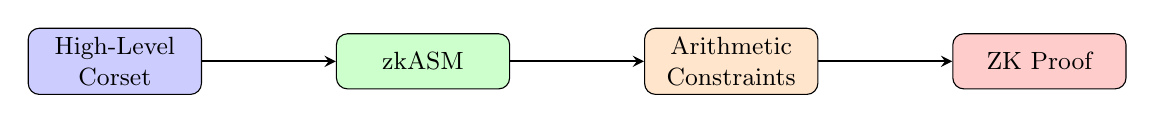
\begin{tikzpicture}[
    node distance=1.2cm,
    box/.style={rectangle, draw, rounded corners, minimum width=2.2cm, minimum height=0.7cm, align=center, font=\small},
    arrow/.style={->, >=stealth, thick}
]
    \node[box, fill=blue!20] (high) {High-Level\\Corset};
    \node[box, fill=green!20, right=of high, xshift=0.5cm] (zkasm) {zkASM};
    \node[box, fill=orange!20, right=of zkasm, xshift=0.5cm] (constraints) {Arithmetic\\Constraints};
    \node[box, fill=red!20, right=of constraints, xshift=0.5cm] (proof) {ZK Proof};

    \draw[arrow] (high) -- (zkasm);
    \draw[arrow] (zkasm) -- (constraints);
    \draw[arrow] (constraints) -- (proof);
\end{tikzpicture}
\end{center}

\vspace{1em}

\begin{columns}
\begin{column}{0.5\textwidth}
\textbf{Advantages}
\begin{itemize}
    \item Direct control over constraints
    \item Predictable constraint counts
    \item Optimized for specific algorithms
    \item Reusable function libraries
\end{itemize}
\end{column}

\begin{column}{0.5\textwidth}
\textbf{Use Cases}
\begin{itemize}
    \item EVM opcode implementations
    \item Cryptographic primitives (Blake2f)
    \item Arithmetic circuits (Division, Modexp)
    \item Bit manipulation routines
\end{itemize}
\end{column}
\end{columns}
\end{frame}

%==============================================================================
\section{Language Features}
%==============================================================================

\begin{frame}[fragile]{Type System}

\begin{columns}
\begin{column}{0.45\textwidth}
\textbf{Unsigned Integer Types}
\begin{table}
\centering
\small
\begin{tabular}{lc}
\toprule
Type & Range \\
\midrule
\texttt{u1} & $[0, 1]$ \\
\texttt{u8} & $[0, 255]$ \\
\texttt{u16} & $[0, 65535]$ \\
\texttt{u32} & $[0, 2^{32}-1]$ \\
\texttt{u128} & $[0, 2^{128}-1]$ \\
\texttt{u256} & $[0, 2^{256}-1]$ \\
\bottomrule
\end{tabular}
\end{table}
\end{column}

\begin{column}{0.55\textwidth}
\textbf{Type Safety}
\begin{itemize}
    \item Compiler verifies bit-width balance
    \item Carry bits explicitly captured
    \item No implicit overflow
\end{itemize}

\vspace{0.5em}
\begin{lstlisting}[style=zkasm]
;; 8-bit + 8-bit = 9-bit result
var carry u1
var result u8
carry, result = a + b  ;; OK!

result = a + b  ;; ERROR: missing carry
\end{lstlisting}
\end{column}
\end{columns}
\end{frame}

%==============================================================================
\begin{frame}[fragile]{Function Declarations}

\begin{lstlisting}[style=zkasm]
fn divide(dividend u16, divisor=1 u16)
    -> (quotient u16, remainder u16) {

    var sum u32
    var witness u16
    var witsum u17

    quotient, remainder, witness, sum, witsum = dividend / divisor
    return
}
\end{lstlisting}

\vspace{0.5em}

\begin{columns}
\begin{column}{0.5\textwidth}
\textbf{Input Parameters}
\begin{itemize}
    \item Named with explicit types
    \item Optional default values (\texttt{=1})
    \item Used for padding in traces
\end{itemize}
\end{column}

\begin{column}{0.5\textwidth}
\textbf{Output Parameters}
\begin{itemize}
    \item Multiple return values
    \item Explicit output types
    \item Optional padding values
\end{itemize}
\end{column}
\end{columns}
\end{frame}

%==============================================================================
\begin{frame}[fragile]{Control Flow}

\begin{columns}
\begin{column}{0.5\textwidth}
\begin{lstlisting}[style=zkasm]
fn counter(n u256, m u256) -> (r u256) {
    var i u256
    var c0, c1 u1

    r = n
    i = m

loop:
    if i == 0 goto exit
    c0, r = r + 1
    c1, i = i - 1
    goto loop

exit:
    return
}
\end{lstlisting}
\end{column}

\begin{column}{0.5\textwidth}
\textbf{Control Flow Constructs}
\begin{itemize}
    \item Labels (\texttt{loop:}, \texttt{exit:})
    \item Conditional jumps (\texttt{if ... goto})
    \item Unconditional jumps (\texttt{goto})
    \item Function return (\texttt{return})
\end{itemize}

\vspace{0.5em}
\textbf{Comparison Operators}
\begin{itemize}
    \item \texttt{==}, \texttt{!=} (equality)
    \item \texttt{<}, \texttt{<=} (less than)
    \item \texttt{>}, \texttt{>=} (greater than)
\end{itemize}
\end{column}
\end{columns}
\end{frame}

%==============================================================================
\begin{frame}[fragile]{Function Calls and Buses}

\begin{columns}
\begin{column}{0.55\textwidth}
\begin{lstlisting}[style=zkasm]
;; Library function
fn square(x u16) -> (r u32) {
    var hi u16
    hi, r = x * x
    return
}

;; Caller function
fn sum_of_squares(a u16, b u16)
    -> (r u32) {
    var sq_a, sq_b u32
    var carry u1

    sq_a = square(a)
    sq_b = square(b)
    carry, r = sq_a + sq_b
    return
}
\end{lstlisting}
\end{column}

\begin{column}{0.45\textwidth}
\textbf{Bus Protocol}
\begin{itemize}
    \item Each function $\to$ unique bus ID
    \item Inputs = address lines
    \item Outputs = data lines
    \item Resolved at link time
\end{itemize}

\vspace{0.5em}
\textbf{Constraints}
\begin{itemize}
    \item Caller writes address
    \item Callee provides data
    \item Lookup verifies match
\end{itemize}
\end{column}
\end{columns}
\end{frame}

%==============================================================================
\section{Compilation Pipeline}
%==============================================================================

\begin{frame}{Pipeline Overview}

\begin{center}
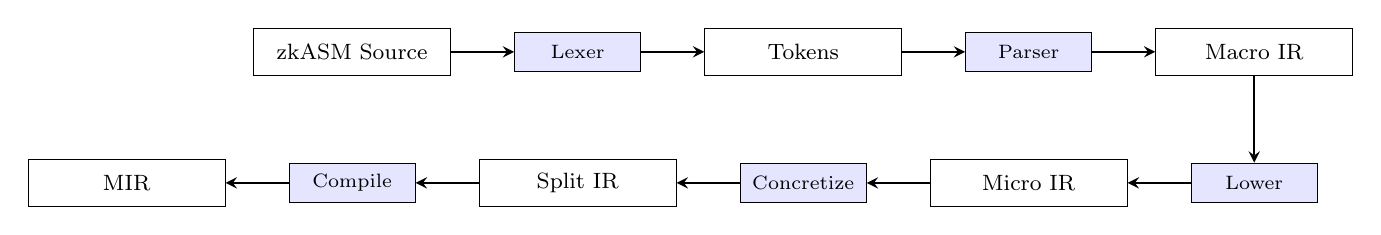
\begin{tikzpicture}[
    node distance=0.8cm,
    box/.style={rectangle, draw, minimum width=2.5cm, minimum height=0.6cm, align=center, font=\footnotesize},
    stage/.style={rectangle, draw, fill=blue!10, minimum width=1.6cm, minimum height=0.5cm, align=center, font=\scriptsize},
    arrow/.style={->, >=stealth, thick}
]
    \node[box] (source) {zkASM Source};
    \node[stage, right=of source] (lex) {Lexer};
    \node[box, right=of lex] (tokens) {Tokens};
    \node[stage, right=of tokens] (parse) {Parser};
    \node[box, right=of parse] (macro) {Macro IR};

    \node[stage, below=of macro, yshift=-0.3cm] (lower) {Lower};
    \node[box, left=of lower] (micro) {Micro IR};
    \node[stage, left=of micro] (concrete) {Concretize};
    \node[box, left=of concrete] (split) {Split IR};
    \node[stage, left=of split] (compile) {Compile};
    \node[box, left=of compile] (mir) {MIR};

    \draw[arrow] (source) -- (lex);
    \draw[arrow] (lex) -- (tokens);
    \draw[arrow] (tokens) -- (parse);
    \draw[arrow] (parse) -- (macro);
    \draw[arrow] (macro) -- (lower);
    \draw[arrow] (lower) -- (micro);
    \draw[arrow] (micro) -- (concrete);
    \draw[arrow] (concrete) -- (split);
    \draw[arrow] (split) -- (compile);
    \draw[arrow] (compile) -- (mir);
\end{tikzpicture}
\end{center}

\vspace{0.5em}

\begin{columns}
\begin{column}{0.5\textwidth}
\textbf{Front-end}
\begin{itemize}
    \item Lexer: Tokenization
    \item Parser: AST construction
    \item Linker: Bus resolution
    \item Validator: Type checking
\end{itemize}
\end{column}

\begin{column}{0.5\textwidth}
\textbf{Back-end}
\begin{itemize}
    \item Lower: Macro $\to$ Micro
    \item Concretize: Field adaptation
    \item Compile: Constraint generation
\end{itemize}
\end{column}
\end{columns}
\end{frame}

%==============================================================================
\begin{frame}{Macro to Micro Lowering}

\begin{columns}
\begin{column}{0.5\textwidth}
\textbf{Macro Instructions}
\begin{itemize}
    \item High-level, user-facing
    \item Complex operations
    \item Control flow abstractions
\end{itemize}

\vspace{0.5em}
\begin{table}
\small
\begin{tabular}{l}
\texttt{Assign} \\
\texttt{Division} \\
\texttt{IfGoto} \\
\texttt{Call} \\
\texttt{Return} \\
\end{tabular}
\end{table}
\end{column}

\begin{column}{0.5\textwidth}
\textbf{Micro Instructions}
\begin{itemize}
    \item Primitive operations
    \item Direct constraint mapping
    \item Explicit control flow
\end{itemize}

\vspace{0.5em}
\begin{table}
\small
\begin{tabular}{l}
\texttt{Assign} (polynomial) \\
\texttt{Skip} (conditional) \\
\texttt{Jmp} (unconditional) \\
\texttt{InOut} (bus I/O) \\
\texttt{Ret}, \texttt{Fail} \\
\end{tabular}
\end{table}
\end{column}
\end{columns}

\vspace{0.5em}

\textbf{Example:} \texttt{if x == 5 goto target} $\Rightarrow$
\begin{enumerate}
    \item \texttt{Skip\{x, 5, skip=1\}} -- skip next if x $\neq$ 5
    \item \texttt{Jmp\{fallthrough\}} -- go to next instruction
    \item \texttt{Jmp\{target\}} -- jump to target
\end{enumerate}
\end{frame}

%==============================================================================
\begin{frame}[fragile]{Vectorization Optimization}

\begin{columns}
\begin{column}{0.5\textwidth}
\textbf{Before Vectorization}
\begin{lstlisting}[style=zkasm]
;; 3 separate instructions
a = x + 1
b = y * 2
c = z - 3
\end{lstlisting}

\vspace{0.5em}
$\Rightarrow$ 3 constraint sets

\vspace{1em}
\textbf{After Vectorization}
\begin{lstlisting}[style=zkasm]
;; 1 merged instruction
{a, b, c} = {x+1, y*2, z-3}
\end{lstlisting}

\vspace{0.5em}
$\Rightarrow$ 1 constraint set
\end{column}

\begin{column}{0.5\textwidth}
\textbf{Merge Conditions}
\begin{itemize}
    \item No register write conflicts
    \item No branch targets between
    \item Sequential in original code
\end{itemize}

\vspace{0.5em}
\textbf{Benefits}
\begin{itemize}
    \item Fewer constraints
    \item Smaller proof size
    \item Faster verification
\end{itemize}
\end{column}
\end{columns}
\end{frame}

%==============================================================================
\section{Field Agnosticity}
%==============================================================================

\begin{frame}{The Field Independence Problem}

\begin{columns}
\begin{column}{0.5\textwidth}
\textbf{Problem}

zkASM programs use types up to \texttt{u256}, but different ZK systems use different finite fields:

\vspace{0.5em}
\begin{table}
\centering
\small
\begin{tabular}{lc}
\toprule
Field & Max Bits \\
\midrule
BLS12-377 & 252 \\
KoalaBear & 30 \\
GF(8209) & 12 \\
\bottomrule
\end{tabular}
\end{table}

\vspace{0.5em}
A 256-bit register doesn't fit in \textit{any} of these fields!
\end{column}

\begin{column}{0.5\textwidth}
\textbf{Solution: Register Splitting}

Split wide registers into limbs:

\begin{center}
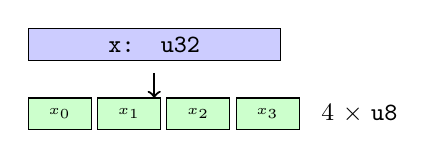
\begin{tikzpicture}[scale=0.8]
    \draw[fill=blue!20] (0,0) rectangle (4,0.5);
    \node at (2, 0.25) {\small \texttt{x: u32}};

    \draw[->, thick] (2, -0.2) -- (2, -0.6);

    \draw[fill=green!20] (0,-1.1) rectangle (1,-0.6);
    \draw[fill=green!20] (1.1,-1.1) rectangle (2.1,-0.6);
    \draw[fill=green!20] (2.2,-1.1) rectangle (3.2,-0.6);
    \draw[fill=green!20] (3.3,-1.1) rectangle (4.3,-0.6);
    \node at (0.5, -0.85) {\tiny $x_0$};
    \node at (1.6, -0.85) {\tiny $x_1$};
    \node at (2.7, -0.85) {\tiny $x_2$};
    \node at (3.8, -0.85) {\tiny $x_3$};

    \node[right] at (4.5, -0.85) {\small 4 $\times$ \texttt{u8}};
\end{tikzpicture}
\end{center}

\vspace{0.3em}
\[
x = x_0 + 2^8 x_1 + 2^{16} x_2 + 2^{24} x_3
\]
\end{column}
\end{columns}
\end{frame}

%==============================================================================
\begin{frame}{Constraint Transformation}

\textbf{Original Constraint} (field-independent):
\[
\texttt{carry} \cdot 2^{16} + \texttt{sum} = a + b
\]

\vspace{0.5em}

\textbf{After Splitting} for 8-bit field max:

\begin{align*}
c_0 \cdot 2^8 + \texttt{sum}_0 &= a_0 + b_0 & \text{(lower byte)}\\
\texttt{carry} \cdot 2^8 + \texttt{sum}_1 &= a_1 + b_1 + c_0 & \text{(upper byte)}
\end{align*}

where $c_0$ is an \textit{internal} carry between limbs.

\vspace{1em}

\begin{center}
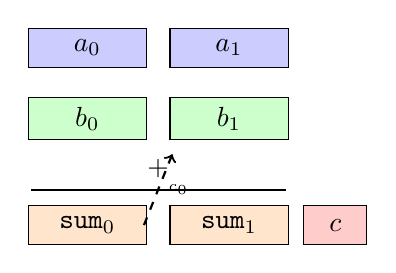
\begin{tikzpicture}[scale=0.9]
    \node[draw, minimum width=1.5cm, minimum height=0.5cm, fill=blue!20] (a0) at (0,1) {$a_0$};
    \node[draw, minimum width=1.5cm, minimum height=0.5cm, fill=blue!20] (a1) at (2,1) {$a_1$};
    \node[draw, minimum width=1.5cm, minimum height=0.5cm, fill=green!20] (b0) at (0,0) {$b_0$};
    \node[draw, minimum width=1.5cm, minimum height=0.5cm, fill=green!20] (b1) at (2,0) {$b_1$};
    \node at (1, -0.7) {$+$};
    \draw[thick] (-0.8,-1) -- (2.8,-1);
    \node[draw, minimum width=1.5cm, minimum height=0.5cm, fill=orange!20] (s0) at (0,-1.5) {$\texttt{sum}_0$};
    \node[draw, minimum width=1.5cm, minimum height=0.5cm, fill=orange!20] (s1) at (2,-1.5) {$\texttt{sum}_1$};
    \node[draw, minimum width=0.8cm, minimum height=0.5cm, fill=red!20] (c) at (3.5,-1.5) {$c$};

    \draw[->, thick, dashed] (0.8,-1.5) -- (1.2, -0.5) node[midway, right] {\tiny $c_0$};
\end{tikzpicture}
\end{center}
\end{frame}

%==============================================================================
\section{Constraint Generation}
%==============================================================================

\begin{frame}[fragile]{Assignment Constraints}

For assignment \texttt{t$_n$, ..., t$_0$ = expr}:

\[
\sum_{i=0}^{n} t_i \cdot 2^{w_i} = \text{eval}(\texttt{expr})
\]

where $w_i = \sum_{j=0}^{i-1} \text{width}(t_j)$.

\vspace{1em}

\begin{columns}
\begin{column}{0.5\textwidth}
\textbf{Example 1: Simple}
\begin{lstlisting}[style=zkasm]
result = a + b
\end{lstlisting}
Constraint: $\texttt{result} = a + b$
\end{column}

\begin{column}{0.5\textwidth}
\textbf{Example 2: With Carry}
\begin{lstlisting}[style=zkasm]
carry, result = a + b
\end{lstlisting}
Constraint: $2^n \cdot \texttt{carry} + \texttt{result} = a + b$
\end{column}
\end{columns}

\vspace{1em}

\textbf{Example 3: Multiplication}
\begin{lstlisting}[style=zkasm]
hi, lo = x * y   ;; x, y: u16, hi, lo: u16
\end{lstlisting}
Constraint: $2^{16} \cdot \texttt{hi} + \texttt{lo} = x \cdot y$
\end{frame}

%==============================================================================
\begin{frame}[fragile]{Division Constraints}

\begin{columns}
\begin{column}{0.5\textwidth}
\begin{lstlisting}[style=zkasm]
q, r, w, sum, witsum = x / y
\end{lstlisting}

\textbf{Generated Constraints:}
\begin{align*}
\texttt{sum} &= q \cdot y + r \\
\texttt{witsum} &= r + w + 1 \\
\texttt{sum} &= x \\
\texttt{witsum} &= y
\end{align*}
\end{column}

\begin{column}{0.5\textwidth}
\textbf{Purpose:}
\begin{itemize}
    \item Eq 1: $q \cdot y + r = \texttt{sum}$
    \item Eq 3: $\texttt{sum} = x$
    \item Together: $x = q \cdot y + r$
\end{itemize}

\vspace{0.5em}
\textbf{Witness proof} ($r < y$):
\begin{itemize}
    \item $w = y - r - 1 \geq 0$
    \item Eq 2: $r + w + 1 = \texttt{witsum}$
    \item Eq 4: $\texttt{witsum} = y$
    \item Thus: $w = y - r - 1$
\end{itemize}
\end{column}
\end{columns}
\end{frame}

%==============================================================================
\begin{frame}{Program Counter Constraints}

\textbf{Multi-line functions} require PC tracking:

\begin{columns}
\begin{column}{0.55\textwidth}
\begin{center}
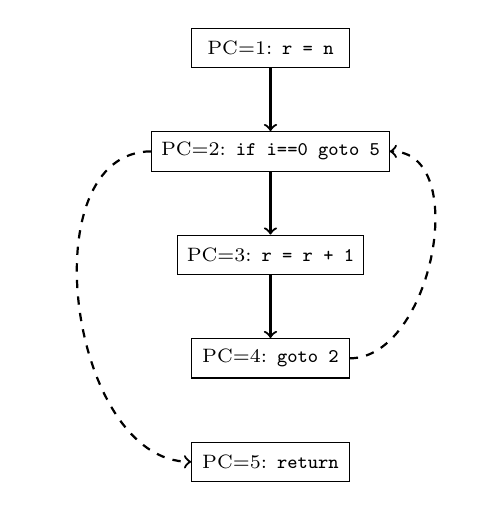
\begin{tikzpicture}[
    node distance=0.8cm,
    box/.style={rectangle, draw, minimum width=2cm, minimum height=0.5cm, align=center, font=\scriptsize}
]
    \node[box] (i0) {PC=1: \texttt{r = n}};
    \node[box, below=of i0] (i1) {PC=2: \texttt{if i==0 goto 5}};
    \node[box, below=of i1] (i2) {PC=3: \texttt{r = r + 1}};
    \node[box, below=of i2] (i3) {PC=4: \texttt{goto 2}};
    \node[box, below=of i3] (i4) {PC=5: \texttt{return}};

    \draw[->, thick] (i0) -- (i1);
    \draw[->, thick] (i1) -- (i2);
    \draw[->, thick] (i2) -- (i3);
    \draw[->, thick, dashed] (i3.east) to[out=0,in=0] (i1.east);
    \draw[->, thick, dashed] (i1.west) to[out=180,in=180] (i4.west);
\end{tikzpicture}
\end{center}
\end{column}

\begin{column}{0.45\textwidth}
\textbf{Constraints:}
\begin{itemize}
    \item Sequential: $\texttt{PC}_{i+1} = \texttt{PC}_i + 1$
    \item Jump: $\texttt{PC}_{i+1} = \texttt{target}$
    \item Return: $\texttt{RET}_i = 1$
\end{itemize}

\vspace{0.5em}
\textbf{Guard formula:}
\[
(\texttt{PC}_i = p) \Rightarrow C_p
\]

Each instruction's constraints are guarded by its PC value.
\end{column}
\end{columns}
\end{frame}

%==============================================================================
\section{Execution Model}
%==============================================================================

\begin{frame}[fragile]{Trace Generation}

\begin{columns}
\begin{column}{0.55\textwidth}
\textbf{Executor State}
\begin{lstlisting}[style=golang]
type State struct {
    pc        uint      // Program counter
    terminal  bool      // Done?
    state     []big.Int // Register values
    io        Map       // I/O for calls
}
\end{lstlisting}

\vspace{0.5em}
\textbf{Execution Loop}
\begin{lstlisting}[style=golang]
for !state.terminal {
    insn := program[state.pc]
    state.pc = insn.Execute(state)
}
\end{lstlisting}
\end{column}

\begin{column}{0.45\textwidth}
\textbf{Trace Structure}

\begin{table}
\centering
\scriptsize
\begin{tabular}{cccc}
\toprule
Row & PC & a & b \\
\midrule
0 & 1 & 5 & 3 \\
1 & 2 & 5 & 3 \\
2 & 3 & 6 & 2 \\
3 & 2 & 6 & 2 \\
4 & 3 & 7 & 1 \\
5 & 2 & 7 & 1 \\
6 & 4 & 8 & 0 \\
\bottomrule
\end{tabular}
\end{table}

Each row = one execution step
\end{column}
\end{columns}
\end{frame}

%==============================================================================
\begin{frame}{Trace Propagation}

\begin{center}
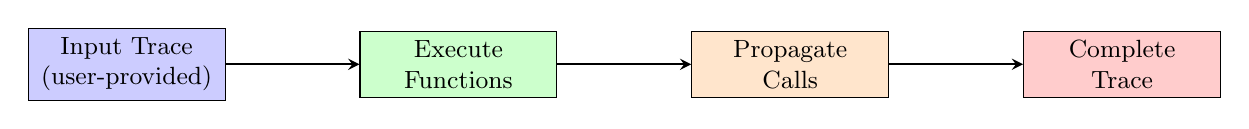
\begin{tikzpicture}[
    node distance=1.2cm,
    box/.style={rectangle, draw, minimum width=2.5cm, minimum height=0.8cm, align=center, font=\small},
    arrow/.style={->, >=stealth, thick}
]
    \node[box, fill=blue!20] (input) {Input Trace\\(user-provided)};
    \node[box, fill=green!20, right=of input, xshift=0.5cm] (exec) {Execute\\Functions};
    \node[box, fill=orange!20, right=of exec, xshift=0.5cm] (prop) {Propagate\\Calls};
    \node[box, fill=red!20, right=of prop, xshift=0.5cm] (output) {Complete\\Trace};

    \draw[arrow] (input) -- (exec);
    \draw[arrow] (exec) -- (prop);
    \draw[arrow] (prop) -- (output);
\end{tikzpicture}
\end{center}

\vspace{1em}

\textbf{Automatic Call Propagation}
\begin{itemize}
    \item User provides instances for top-level functions
    \item Executor runs functions, recording all internal calls
    \item Called functions automatically get their instances generated
    \item Final trace includes all function instances
\end{itemize}

\vspace{0.5em}

\textbf{Instance Caching}
\begin{itemize}
    \item Same inputs $\Rightarrow$ cached outputs
    \item Avoids redundant computation
    \item Thread-safe with mutex protection
\end{itemize}
\end{frame}

%==============================================================================
\section{Integration}
%==============================================================================

\begin{frame}{Mixed Program Model}

\begin{center}
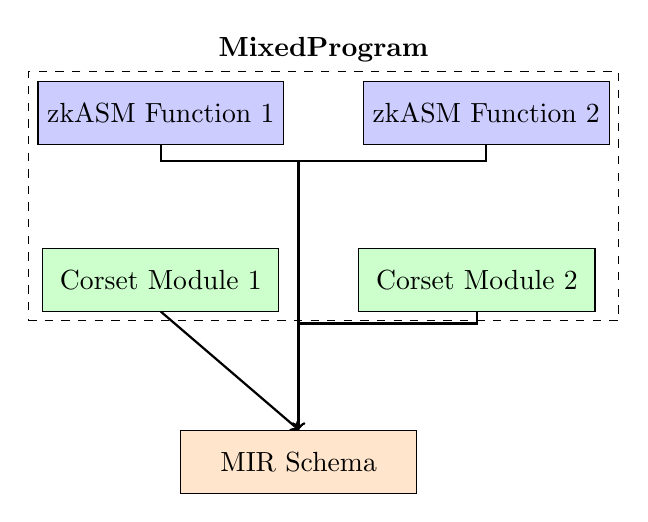
\begin{tikzpicture}[
    node distance=1cm,
    box/.style={rectangle, draw, minimum width=3cm, minimum height=0.8cm, align=center},
    container/.style={rectangle, draw, dashed, minimum width=7cm, minimum height=2cm}
]
    \node[box, fill=blue!20] (zkasm1) {zkASM Function 1};
    \node[box, fill=blue!20, right=of zkasm1] (zkasm2) {zkASM Function 2};
    \node[box, fill=green!20, below=of zkasm1, yshift=-0.3cm] (corset1) {Corset Module 1};
    \node[box, fill=green!20, right=of corset1] (corset2) {Corset Module 2};

    \node[container, fit=(zkasm1)(zkasm2)(corset1)(corset2), label=above:{\textbf{MixedProgram}}] {};

    \node[box, fill=orange!20, below=of corset1, xshift=1.75cm, yshift=-0.5cm] (mir) {MIR Schema};

    \draw[->, thick] (zkasm1.south) -- ++(0,-0.2) -| (mir.north);
    \draw[->, thick] (zkasm2.south) -- ++(0,-0.2) -| (mir.north);
    \draw[->, thick] (corset1.south) -- (mir.north);
    \draw[->, thick] (corset2.south) -- ++(0,-0.15) -| (mir.north);
\end{tikzpicture}
\end{center}

\vspace{0.5em}

\begin{columns}
\begin{column}{0.5\textwidth}
\textbf{zkASM Functions}
\begin{itemize}
    \item Compiled from \texttt{.zkasm} files
    \item Explicit register control
    \item Optimized constraint generation
\end{itemize}
\end{column}

\begin{column}{0.5\textwidth}
\textbf{Corset Modules}
\begin{itemize}
    \item Compiled from \texttt{.lisp} files
    \item High-level constraint language
    \item Shared schema namespace
\end{itemize}
\end{column}
\end{columns}
\end{frame}

%==============================================================================
\begin{frame}{Bus Communication}

\begin{center}
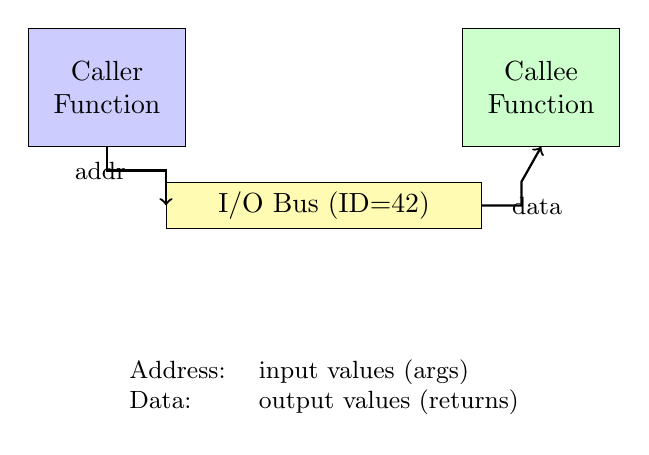
\begin{tikzpicture}[
    node distance=2cm,
    func/.style={rectangle, draw, minimum width=2cm, minimum height=1.5cm, align=center},
    bus/.style={rectangle, draw, fill=yellow!30, minimum width=4cm, minimum height=0.5cm}
]
    \node[func, fill=blue!20] (caller) {Caller\\Function};
    \node[func, fill=green!20, right=of caller, xshift=1.5cm] (callee) {Callee\\Function};
    \node[bus] (bus) at ($(caller)!0.5!(callee) + (0,-1.5)$) {I/O Bus (ID=42)};

    \draw[->, thick] (caller.south) -- ++(0,-0.3) -| node[near start, left] {\small addr} (bus.west);
    \draw[->, thick] (bus.east) -| node[near start, right] {\small data} ++(0.5,0.3) -- (callee.south);

    \node[below=of bus, yshift=0.5cm, font=\small] {
        \begin{tabular}{ll}
        Address: & input values (args) \\
        Data: & output values (returns)
        \end{tabular}
    };
\end{tikzpicture}
\end{center}

\vspace{0.5em}

\textbf{Bus Protocol}
\begin{itemize}
    \item Each function assigned unique bus ID at link time
    \item Caller writes inputs to address lines
    \item Callee provides outputs on data lines
    \item Lookup constraint verifies (addr, data) pairs exist
\end{itemize}
\end{frame}

%==============================================================================
\section{Summary}
%==============================================================================

\begin{frame}{Key Takeaways}

\begin{columns}
\begin{column}{0.5\textwidth}
\textbf{Language Features}
\begin{itemize}
    \item Strong type system (u1-u256)
    \item Explicit carry/overflow handling
    \item Clean function composition
    \item Field-agnostic programming
\end{itemize}

\vspace{0.5em}
\textbf{Compilation}
\begin{itemize}
    \item Multi-stage pipeline
    \item Macro $\to$ Micro lowering
    \item Vectorization optimization
    \item Automatic register splitting
\end{itemize}
\end{column}

\begin{column}{0.5\textwidth}
\textbf{Constraint Generation}
\begin{itemize}
    \item Direct polynomial mapping
    \item PC-guarded multi-line functions
    \item Division with witness proofs
    \item Bus-based function calls
\end{itemize}

\vspace{0.5em}
\textbf{Execution}
\begin{itemize}
    \item Deterministic trace generation
    \item Automatic call propagation
    \item Instance caching
    \item Thread-safe execution
\end{itemize}
\end{column}
\end{columns}

\vspace{1em}
\begin{center}
\textbf{zkASM enables precise, portable, and efficient ZK circuit programming}
\end{center}
\end{frame}

%==============================================================================
\begin{frame}{Package Structure}

\begin{columns}
\begin{column}{0.5\textwidth}
\textbf{Source Organization}

\texttt{pkg/asm/}
\begin{itemize}
    \item \texttt{assembler/} -- lexer, parser, linker, validator
    \item \texttt{compiler/} -- constraint generation
    \item \texttt{io/} -- core abstractions
    \begin{itemize}
        \item \texttt{macro/} -- macro instructions
        \item \texttt{micro/} -- micro instructions
    \end{itemize}
    \item \texttt{program/} -- module wrappers
\end{itemize}
\end{column}

\begin{column}{0.5\textwidth}
\textbf{Test Coverage}
\begin{itemize}
    \item 34+ unit test files
    \item Arithmetic operations
    \item Control flow patterns
    \item Function calls
    \item Bit manipulation
    \item Field-specific tests
\end{itemize}

\vspace{0.5em}
\textbf{Benchmarks}
\begin{itemize}
    \item EVM opcodes
    \item Blake2f
    \item Division/Modexp
    \item Shift operations
\end{itemize}
\end{column}
\end{columns}
\end{frame}

%==============================================================================
\begin{frame}{Questions?}
\begin{center}
\vspace{2em}
{\Huge Questions?}

\vspace{3em}
{\large \texttt{github.com/consensys/go-corset}}
\end{center}
\end{frame}

\end{document}
